\documentclass{trkut}% Reaalkooli vormistus. Muidu "report" või "article".
\usepackage[style=trkut]{biblatex}% Kasutatud kirjanduse genereerimine
\usepackage{mleftright, braket}
\addbibresource{viited_kaarel_kivisalu.bib}% Viidete info fail
\defbibheading{bibliography}{\addchap{#1}}% Lisame kasutatud materjalid sisukorda

\pealkiri{Gravitatsiooni mõju kera soojusmahtuvusele}
\autor{Kaarel Kivisalu}
\klass{11. a}
\juhendaja{prof Jaan Kalda \\ õp Toomas Reimann}
\toggletrue{mitujuhendajat}% Uncomment kui on mitu juhendajat

\DeclareMathOperator{\tr}{tr}
\DeclareMathOperator{\erf}{erf}
\NewDocumentCommand{\op}{o m}{\IfNoValueTF{#1}{\hat{#2}}{\hat{#2}^{#1}}}
\renewcommand\bra[1]{{\langle{#1}|}}
\renewcommand\ket[1]{{|{#1}\rangle}}
\renewcommand\Bra[1]{\mleft\langle#1\mright|}
\renewcommand\Ket[1]{\mleft|#1\mright\rangle}


\begin{document}
\maketitle% Tiitelleht
\tableofcontents% Sisukord
\addchap{Sissejuhatus}
\nummerdame% See käsk peab olema õigeks nummerdamiseks kohe peale sissejuhatust
I rahvusvahelisel füüsikaolümpiaadil 1967. aastal oli järgnev probleem \cite{ipho67}:

\textit{Kaks homogeenset ühesugust kera on sama algtemperatuuriga. Üks kera on liikumatult horisontaalse tasandil, teine ripub niidi küljes. Mõlemale kerale antakse võrdne soojushulk. Kas kerade lõpptemperatuur on sama või mitte. Soojuskadudega mitte arvestada.}

Käesolevas töös uuritakse konkreetsete potentsiaalide korral konstantse gravitatsioonvälja mõju kera soojusmahtuvusele. Konstantse gravitatsioonivälja potentsiaal on lineaarne. Vaadatakse soojusmahtuvuse erinevust juhtudel, kui on ainult kera potentsiaal ja kera potentsiaalile on lisatud lineaarne gravitatsioonivälja potentsiaal.

Töös on analüüsitud kuuppolünoompotentsiaali häirituse meetodil ja kahest lineaarsest funktsioonist koosnevat potentsiaali kvaasi-klassikaliselt. Samuti on näidatud, et osade potentsiaalide korral ei mõjuta gravitatsioon soojusmahtuvust.

Varem on uuritud gravitatsiooni mõju metallkera soojusmahtuvusele üldjuhul. Leiti üldine seos soojusmahtuvuse, temperatuuri, gravitatsioonivälja tugevuse ja lineaarse soojuspaisumisteguri vahel. Saadud tulemust on eksperimentaalselt väga raske kinnitada, kuna gravitatsiooni mõju on väga väike. Konkreetsete potentsiaalide läbivaatamine tõstaks ka varem leitud mudeli usaldusväärsust.

Uurimistöö hüpotees on, et sõltuvalt potentsiaalist võib gravitatsioon nii tõsta kui ka langetada keha soojusmahtuvust.

\chapter{Teoreetiline osa}

\section{Tavapärane lahendus}

Tavapärane lahendus põhineb soojuspaisumisega seotud erinevustel. Kerale $A$ soojust andes see paisub ja selle massikese tõuseb. Järelikult peab osa kerale A antavast soojushulgast kuluma kera massikeskme gravitatsioonilise potentsiaalse energia tõstmiseks ja lõpptemperatuur on madalam algsest. Vastupidiselt, kera $B$ massikese langeb soojuspaisumise tõttu ja energiat saadakse juurde, järelikult on kera $B$ lõpptemperatuur kõrgem.

Pannakse ka kirja tavapärasele lahendusele vastavad valemid. Olgu kerade soojusmahtuvus $C_0$ gravitatsioonivälja puudumisel. Tavapärase lahenduse korrale, kui kera A soojendatakse, siis selle massikese tõused $dR=\alpha R \, dT$ võrra, kus $dT$ on temperatuuri tõus, $\alpha$ on soojuspaisumistegur ja $R$ on kera raadius. Kera saab potentsiaalse energia $d\Phi = mg \, dR$, kus $m$ on keha mass ja $g$ on raskuskiirendus. Järelikult, kui soojushulk \(\delta Q\) antakse süsteemile, siis saadakse, et
\begin{equation}
    \delta Q = C_0 \, dT + mg \, dR = C_0 \, dT + mg\alpha R \, dT = (C_0 +  mg\alpha R) dT.
\end{equation}
See on ekvivalentne väitega, et kera \(A\) soojusmahtuvus on:
\begin{equation}
    C_A = C_0 + mg\alpha R.
\end{equation}
Analgoselt saame, et kera \(B\) soojusmahtuvus on
\begin{equation}
    C_B = C_0 - mg\alpha R.
\end{equation}
Enamiku materjalide jaoks on \(\alpha > 0\), millest tulenevalt \(C_A>C_B\). Järelikult on tavapärase lahenduse kohaselt kera \(A\) lõpptemperatuur madalam kera \(B\) lõpptemperatuurist.

\section{Tavapärane lahendus ja selle termodünaamika II seaduse rikkumine}

Tavapärases lahenduses kaudselt eeldatakse, et keha siseenergia \(U\) ja raadius \(R\) sõltuvad ainult temperatuurist \(T\), mitte aga raskuskiirendusest \(g\). Vaadeltakse järgnevat tsüklit: pall asub horisontaalsel külmal tasandil temperatuuriga \(T_1\); pall ühendatakse soojema reservaariga, mille temperatuur \(T_2=T_1+dT>T_1\); pall riputatakse nööri külge ja horisontaalne tasand eemaldatakse; pall ühendatakse külma revervuaariga, mille temperatuur on \(T_1\). Selle protsessi kasutegur on tehtud töö ja neeldunud soojuse suhe ning avaldub kujul \cite{palma15}
\begin{equation}
    \eta = \frac{2mg\alpha R}{C_0+mg\alpha R}.
\end{equation}
Kasutegur \(\eta\) ei sõltu \(dT\) suurusest. Termodünaamika teist seadus saab sõastada järgnevalt: iga tsükkel, mis töötab ainult temperatuuride \(T_1\) ja \(T_2\) juures ei saa olla effektiivsem Carnot' tsüklist, mis töötab samade temperatuuride juures. Carnot' tsükli efektiivsus on
\begin{equation}
    \eta_{Carnot'} = \frac{dT}{T_2}
\end{equation}
Järelikult, kui \(dT\) on piisavalt väike, siis on palliga tsükli kasutegur suurem Carnot' tsükli kasutegurist. Teisisõnu rikub tavapärane lahendus termodünaamika II seadust.
\begin{figure}[h]
    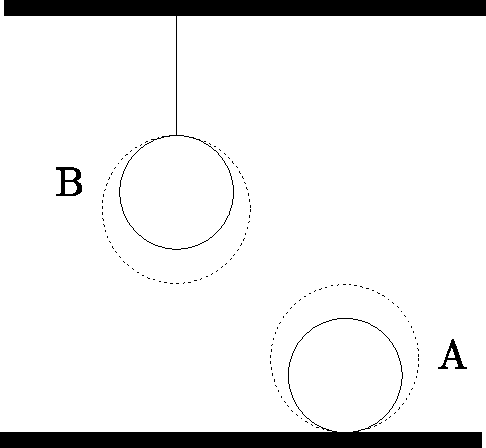
\includegraphics[width=0.5\textwidth]{joonis1.pdf}
    \caption{Probleemi ülesehitus}
    \allikas{\protect\cite{palma15}}
    \label{iphojoonis}% Selle järgi viidatakse, see rida peab olema pärast \caption
\end{figure}

\section{Statistiline mehaanika}

Kasutades statistilise mehaanika meetodeid on võimalik leida kera soojusmahtuvuse sõltuvus gravitatsioonist \parencite[test]{palma15}:
\begin{equation}
    \frac{\partial C(g,T)}{\partial g} = -mTY \left( \alpha^2 + \frac{\partial \alpha}{\partial T} \right),
\end{equation}
kus \(C\) on soojusmahtuvus, \(g\) on raskuskiirenuds, \(m\) on kera mass, \(T\) on kera temperatuur, \(Y\) on massikeskme kõrgus, \(\alpha\) on lineaarne soojuspaisumistegur.

%\section{Schroedingeri vorrand}
%
%Ajast sõltumatu Scröendingeri võrrand ühes dimensioonis avaldub kujul \cite{griffiths05}
%\begin{equation}
%    \op{H} \Psi = E \Psi,
%\end{equation}
%kus \(E\) on süsteemi koguenergia ja
%\begin{equation}
%    \op{H}=-\frac{\hbar^2}{2m}\frac{d^2}{dx^2}+V(x).
%\end{equation}

\section{Energiatasemed ja soojusmahtuvus}

Kanoonilise ansambli jaoks, mis on kvantmehaaniline ja diskreetne, on kanooniline statistiline summa \(Z\) defineeritud kui jälg Boltzmanni tegurist \cite{kardar07}:
\begin{equation}
    Z=\tr(e^{-\beta \op{H}})=\sum_{n} e^{-\beta E_n}.
\end{equation}
Keskmine energia \(U\) avaldub kui \cite{kardar07}
\begin{equation}
    U=- \frac{\partial \ln Z}{\partial \beta}.
\end{equation}
Soojusmahtuvus on defineeritud kui
\begin{equation}
    C=\frac{\partial U}{\partial T}.
\end{equation}
Eelnevatest võrranditest on lihtne näha, et
\begin{equation}
    \frac{\partial C}{\partial g}=- \frac{\partial}{\partial g}  \frac{\partial}{\partial T} \frac{\partial}{\partial \beta} \ln {\sum_{n} e^{-\beta E_n}}.
\end{equation}

\section{Kvaasi-klassikaline lähendus}

Schrödingeri võrrandi
\begin{equation}
    -\frac{\hbar^2}{2m}\frac{d^2\psi}{dx^2}+V(x)\psi=E\psi
\end{equation}
saab ümber kirjutada järgnevalt:
\begin{equation}
    \frac{d^2 \psi}{dx^2}= - \frac{p^2}{\hbar^2}\psi,
\end{equation}
kus
\begin{equation}
    p(x) \equiv \sqrt{2m[E-V(x)]}
\end{equation}
on klassikaline valem osakese impulsi jaoks koguenergiaga $E$ ja potentsiaalse energiaga $V(x)$.
Piirkonnas, kus $E>V(x)$, on $p(x)$ reaalne. Seda piirkonda kutsutakse \enquote{klassikaliseks}, kuna klasskikaliselt on osake piiratud selles piirkonnas.
Üldiselt on $\psi$ kompleksfunktsioon, mida saab avaldada klassikalises piirkonnas amplituudi $A(x)$ ja faasi $\phi(x)$ kaudu, mis mõlemad on reaalsed \parencite[316]{griffiths05}:
\begin{equation}
    \psi(x)=A(x)e^{i\phi(x)}.
\end{equation}
Eeldades, et amplituud $A$ muutub aeglaselt\footnote{Täpsemalt eeldatakse, et $A''/A\ll(\phi ')^2$ ja $A''/A\ll p^2/\hbar^2$.}, avaldub lainefunktsioon klassikalises piirkonnas kujul \parencite[316-318]{griffiths05}
\begin{equation}
    \psi = \frac{C_1}{\sqrt{p(x)}}e^{\frac{i}{\hbar}\int p(x)\, dx} +\frac{C_2}{\sqrt{p(x)}}e^{-\frac{i}{\hbar}\int p(x)\, dx},
    \label{eq:kvaasik1}
\end{equation}
kus $C_1$ ja $C_2$ on kompleksarvulised konstandid.
Valemi \eqref{eq:kvaasik1} saab ka kirja panna kujul \parencite[446]{shankar94}
\begin{equation}
    \psi(x)=\frac{A}{\sqrt{p(x)}} \cos \left[ \frac{1}{\hbar}\int p(x)\, dx + B \right],
    \label{eq:kvaasik2}
\end{equation}
kus $A$ ja $B$ on reaalsed parameetrid.
Kahjuks ei kehti \eqref{eq:kvaasik2} kui $E \approx V(x)$, kuna $\sqrt{p(x)} \to 0$. Olgu $V(x_1)=V(x_2)=E$, $x_1<x_2$ ja lõigul $(x_1, x_2)$ on $V(x)<E$.
On siiski võimalik vaadeldes lainefunktsiooni $x_1$ lähedal näidata, et lõigul $(x_1, x_2)$ on lainefunktsioon järgmine \parencite[167-170]{landau05}:
\begin{equation}
    \psi(x)=\frac{A}{\sqrt{p(x)}} \cos \left[ \frac{1}{\hbar}\int_{x_1}^{x} p(x)\, dx - \frac{\pi}{4} \right],
\end{equation}
kui $x_2$ lähedal on lainefunktsioon
\begin{equation}
    \psi(x)=\frac{A'}{\sqrt{p(x)}} \cos \left[ \frac{1}{\hbar}\int_{x_2}^{x} p(x)\, dx + \frac{\pi}{4} \right].
\end{equation}
Selleks, et need kaks lahendit ühtiksid, peavad $A$ ja $A'$ olema sama magnituudiga ja koosinuste faaside vahe peab olema $\pi$ kordne \parencite[446]{shankar94}:
\begin{equation}
    \frac{1}{\hbar}\int_{x_1}^{x} p(x)\, dx - \frac{1}{\hbar}\int_{x_2}^{x} p(x)\, dx - \frac{\pi}{2} = n\pi
\end{equation}
või
\begin{equation}
    \int_{x_1}^{x_2} p(x)\, dx =\left(n+\frac{1}{2}\right)\pi \hbar.
\end{equation}



\section{Ajast sõltumatu häiritusteooria}

Schrödingeri võrrandit täpselt lahendada on võimalik ainult lihtsamatel juhtudel, keerulisemate juhtude jaoks on vaja teha lähendusi.
Ajast sõltumatu häiritusteooria (edaspidi häiritusteooria) on lähendusmeetod, mida saab rakendada järgnevas olukorras: teades lahendit hamiltoniaani $\op[0]{H}$ omaväärtusülesandele (ingl \textit{eigenvalue problem}), tahetakse leida lahendit $\op{H}=\op[0]{H}+\op[1]{H}$, kus $\op[1]{H}$ on suhteliselt väike võrreldes $\op[0]{H}$-ga.
Eeldatakse, et iga $\op[0]{H}$ kidumata omaketi (ingl \textit{eigenket}) $\Ket{n^0}$ omaväärtusega $E_n^0$ jaoks leidub $\op{H}$ kidumata omaket $\Ket{n}$ omaväärtusega $E_n$. Siis eeldades, et $H$ omaketid ja omaväärtused võib kirja panna häiritusseerias \parencite[451]{shankar94}:
\begin{align}
    \Ket{n}&=\Ket{n^0}+\Ket{n^1}+\Ket{n^2}+... \\
    E_n&=E_n^0+E_n^1+E_n^2+...
\end{align}
Iga liikme ülaindeks $k$ näitab millise $\op[1]{H}$ astmega eeldatakse, et iga liige on võrdeline.
Selleks, et leida liikmeid $\Ket{n}$ ja $E_n$ arenduses, alustatakse omaväärtusvõrrandiga \parencite[451]{shankar94}:
\begin{equation}
    \op{H}\Ket{n}=E_n\Ket{n}
\end{equation}
või
\begin{equation}
    \big(\op[0]{H} + \op[1]{H}\big)\left(\Ket{n^0}+\Ket{n^1}+...\right)=\left(E_n^0+E_n^1+...\right) \left(\Ket{n^0}+\Ket{n^1}+...\right).
    \label{terms}
\end{equation}
Vaadates võrrandis \eqref{terms} nullindat järku liikmeid saadakse võrrand
\begin{equation}
    \op[0]{H}\Ket{n^0}=E_n^0\Ket{n^0}.
\end{equation}
Eelduse järgi on see võrrand lahendatud ja omaket $\Ket{n^0}$ ja omaväärtused $E_n^0$ on teada. Vaadates võrrandis \eqref{terms} esimest järku liikmeid saadakse võrrand
\begin{equation}
    \op[0]{H}\Ket{n^1} + \op[1]{H}\Ket{n^0} = E_n^0\Ket{n^1} + E_n^1\Ket{n^0}
\end{equation}

%Häirituse teooria diskreetse spektrumi jaoks saab formuleerida järgnevalt. Eeldatakse, et on teada diskreetse spektri omaväärtused (ingl  \textit{eigenvalues}) \(E_0^{(0)}\) ja omafunktsioonid (ingl \textit{eigenfunctions}) \(\phi^0\) häitimata operaatori \(H_0\) jaoks, st et on teada võrrandi
%\begin{equation}
%    H_0 \psi=E_0 \psi
%\end{equation}
%täpsed lahendid. Soovitakse leida ligikaudseid lahendeid võrrandile
%\begin{equation}
%    \op{H} \psi=(H_0+V)\psi=E\psi,
%\end{equation}
%st ligikaudesd avaldised häiritud operaatori \(\op{H}\) omafunktsioonide \(\phi_n\) ja omaväärtuste \(E_n\) väärtused.\parencite{landau05}

\chapter{Praktiline osa}

Käesolevas osas leitakse konkreetsetele võimalikele kera potentsiaalidele vastavad soojusmahtuvuse sõltuvused gravitatsioonist, kus gravitatsiooni potentsiaal on võetud lineaarseks sõltuvalt ühest koordinaadist. Kuigi tegelik kera potentsiaal on keeruline võib anda konkreetne potentsiaal küllaltki täpse lahendi.

\section{Tükiti lineaarne potentsiaal}
Vaadeltakse potentsiaali kujuga
\begin{equation}
    V(x)=\begin{cases}
        (-a+mg)x, & x<0,\\
        (b+mg)x, & x\ge0,
    \end{cases}
\end{equation}
kus $a$ ja $b$ on positiivsed reaalarvulised konstandid ning $-a+mg<0$ ja $b+mg>0$.
Kvaasi-klassikalises lähenduses saame leida vastava energiatasemed:
\begin{equation}
    \left( n+\frac{1}{2}\right)\pi \hbar = \int_{x_1}^{0} \sqrt{2m[E_n-(-a+mg)x]}\, dx + \int_{0}^{x_2} \sqrt{2m[E_n-(b+mg)x]} \, dx,
\end{equation}
kus \(n \in \{0, 1, 2, ...\}\), \(x_1=\frac{E_n}{-a+mg}\) ja \(x_2=\frac{E_n}{b+mg}\). Integreerides saadakse, et
\begin{align}
    \left(n+\frac{1}{2}\right)\pi \hbar &= \sqrt{2m}\left.\left[-\frac{2(E_n-(-a-mg)x)^\frac{2}{3}}{3(-a+mg)}\right]\right|^0_{x_1} + \sqrt{2m}\left.\left[-\frac{2(E_n-(b-mg)x)^\frac{2}{3}}{3(b+mg)}\right]\right|^{0}_{x_2} \notag \\
    &= -\frac{2\sqrt{2m}E_n^{\frac{3}{2}}}{3(-a+mg)}+\frac{2\sqrt{2m}E_n^{\frac{3}{2}}}{3(b+mg)}.
\end{align}
$E_n$ avaldades saadakse, et
\begin{equation}
    E_n =\left[\frac{3\pi}{2\sqrt{2}} \frac{\hbar}{\sqrt{m}} \frac{(-a+mg)(b+mg)}{a+b}\right]^{\frac{2}{3}} \left(n+\frac{1}{2}\right)^{\frac{2}{3}} . \label{tukene}
\end{equation}
Asendades võrrandisse \eqref{tukene} $c=\left[\frac{3\pi}{2\sqrt{2}} \frac{\hbar}{\sqrt{m}} \frac{(-a+mg)(b+mg)}{a+b}\right]^{\frac{2}{3}}$ avaldub statistiline summa järgnevalt:
\begin{equation}
    Z=\sum_{n=0}^{\infty} e^{-\beta c \left(n+\frac{1}{2}\right)^\frac{2}{3}}.
\end{equation}
Kui $\beta c\ll 1$, siis saab summa asendada integraaliga ja $n+\frac{1}{2}\approx n$:
\begin{equation}
    Z=\sum_{n=0}^{\infty} e^{-\beta c \left(n+\frac{1}{2}\right)^\frac{2}{3}} \approx \int_0^\infty e^{-\beta c n^\frac{2}{3}} \, dn = \left.\left[ \frac{3\sqrt{\pi}  \erf{\left( {n}^\frac{1}{3} \sqrt{\beta c}\right)} }{4 (\beta c)^\frac{3}{2}}-\frac{3n^\frac{1}{3} e^{-\beta cn^\frac{2}{3}}}{2 \beta c }\right]\right|^{\infty}_{0}=\frac{3\sqrt{\pi}}{4(\beta c)^\frac{3}{2}} .
\end{equation}

\section{Tükiti paraboolne potentsiaal}

\begin{equation}
    \frac{\sqrt{m} \left( \sqrt{2} {g}^{2} m^2 + {{2}^{\frac{5}{2}}}\, {E_n} a\right)  \arcsin\left( \frac{\sqrt{{{g}^{2}}\, {{m}^{2}}+4 {E_n} a} \sqrt{{{g}^{2}}\, {{m}^{4}}+4 {E_n} a\, {{m}^{2}}}}{{{g}^{2}}\, {{m}^{3}}+4 {E_n} a m}\right) }{4 {{a}^{\frac{3}{2}}}}=\ensuremath{\pi}  \left( n+\frac{1}{2}\right)  \hbar
\end{equation}

\section{Häiritusega harmooniline ostsillaator}
Vaadeldakse järgnevat hamiltooninit
\begin{equation}
    \op{H}=\op[0]{H}+\op[1]{H},
\end{equation}
kus
\begin{equation}
    \op[0]{H}=\frac{\op{p}^2}{2m}+\frac{m\omega^2 \op{x}^2}{2}
\end{equation}
ja
\begin{equation}
    \op[1]{H}=mg\op{x}
\end{equation}
<++>
Lahendid saame leida häirituse meetodiga. On lihtne potentsiaali
\begin{equation}
    V(x)=\frac{m\omega^2 x^2}{2}+mgx
\end{equation}
omaväärtused, kui teha asendus \(y=x+\frac{g}{\omega^2}\). Saadakse, et
\begin{equation}
    E_n=\left(n+\frac{1}{2}\right) \hbar \omega - \frac{1}{2}\frac{mg^2}{\omega^2}.
\end{equation}

\addchap{Kokkuvõte}

% \nocite{*}
\printbibliography
\kinnitusleht

    \end{document}
